%!TEX root = ../swiatlow_thesis.tex
\label{chapter:susy}

\section{The Problem of the Standard Model}
\label{chapter:susy:problems}

It is somewhat incongruous to say that the SM has problems after describing the huge degree of its success in Chapter~\ref{chapter:sm}, but there are clear tensions in the model which point to signs of potential new extensions. The following sections describe some of these shortcomings.

\subsection{The Pursuit of Beauty, or Naturalness}

The process of developing a fundamental theory of nature is intended to be simplifying: for example, the development of the parton model and QCD simplified the eight-fold way and the complicated sea of hadrons  that came before it. The core of this simplification was the realization of a symmetry-- the $SU(3)$ of color-- which reduced a complicated system to a more simple one. There is an element to this that a physicist might call beautiful: the realization of an underlying simple pattern which explains something complicated. In that sense, there should be very few accidents in a theory: there should be a \textit{reason} for things to be the way they are. For example, there are no accidental, or ad-hoc terms in a Lagrangian: we include all relevant terms allowed by the symmetry groups, and derive the consequences. The symmetry groups are the reason that the Lagrangians look the way they do.

In this same sense, constants in the theory can be arbitrary, but requiring them to be \textit{arbitrarily precise} is something of an aesthetic problem: the theory should not care if the mass of the up or down quark were different by $50\%$, for example. However, there is exactly one such finely tuned mass in the Standard Model-- $m_h$, the mass of the Higgs boson. 

As discussed in Section~\ref{chapter:sm:qcd:freedom}, higher-order terms caused by loop diagrams induce corrections to constants, such as masses and coupling constants, through the process of renormalization. The Higgs boson's mass is not immune, and since the Higgs couples to all particles (except gluons) via either electroweak symmetry breaking terms or the Yukawa couplings to matter, in principle all of these particles can create loops which correct the Higgs mass. Because it has the largest coupling, the loop involving the top quark-- pictured in Figure~\ref{fig:susy:higgs-loop}--  has the largest contribution out of all these terms. \editnote{cite Martin} The correction, in fact, goes as:
%
\begin{equation}
\Delta m_H^2 = - \frac{|y_T|^2}{8\pi^2}\Lambda_\mathrm{UV}^2 + \ldots
\end{equation}
%
where $y_T$ is the top Yukawa coupling, and $\Lambda_\mathrm{UV}$ is the UV cutoff of the theory. This correction grows quadratically with the cut-off scale: if the SM is the only theory of nature up to the Planck scale (where quantum gravity takes effect, thereby signficantly changing the appropriate physical description), then the correction is in fact proportional to $M_\mathrm{Planck}^2$. The observed Higgs boson has a mass of 126 GeV, which is quite far from $M_\mathrm{Planck} = 1.22\times 10^{19}$~GeV: the only way to reconcile the measurement with the observation, is to set $m_0$, the bare Higgs mass before corrections, to a \textit{precise} value such that $m_0$ and $\Delta m_H^2$ cancel perfectly to 126 GeV. Thus, the SM requires the bare mass to be precisely defined to 1 part in $10^{-19}$-- a value so precisely tuned that it seems unlikely to have arisen by chance. 

%%%%%%%%%%%%%%%%

\begin{figure}
\centering
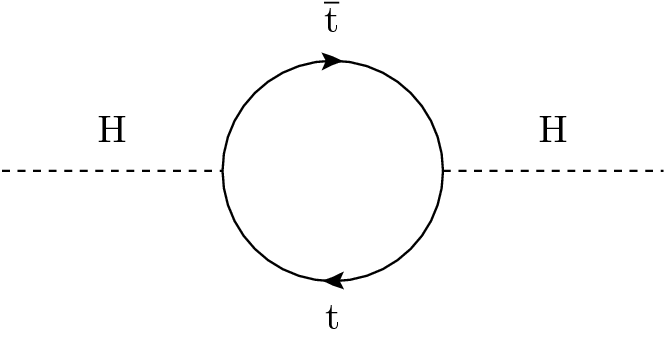
\includegraphics[width=0.7\textwidth]{higgs-loop.png}
\label{fig:susy:higgs-loop}
\caption{An example of a loop diagram which renormalizes the Higgs mass. Courtesy of PyFeyn.}
\end{figure}

%%%%%%%%%%%%%%%%  

Thus, the mass of the Higgs boson is not like that of other constants in the theory-- it is not arbitrary, like the masses of the quarks or leptons-- and the observed mass is substantially outside of the preferred range (at the Planck scale).  The SM's solution to this issue-- a precise cancelling of terms-- has an aesthetic penalty: there is no \textit{reason} for this cancellation in the SM, only blind luck. Physicists say that this kind of solution lacks \textit{naturalness}: there is no underlying symmetry or simplification to explain it, and only a complication of a very particular number.



\subsection{Unification}

Another aesthetic criticism of the SM lies in its separation of forces. The electroweak model is seen as particularly elegant because the electroweak symmetry, though broken at low energies by the Higgs mechanism, provides a unifying structure to two initially disparate forces (electomagnetism and the weak force). One natural question is whether some higher symmetry group unifies all the SM forces, and not just the electroweak. 


\subsection{Dark Matter}

One final motivation for the existence of physics beyond the SM is based on firm experimental ground and not just aesthetic preference: this is the presence of dark matter in the universe. 

\section{Supersymmetry: The Solution?}

These three shortcomings of the SM motivate the need for new theories-- but it turns out that one particularly interesting theory solves all three problems at once. This theory, called \textit{supersymmetry}, solves the problems of the SM in a very elegant way, by introducing a new symmetry between bosons and fermions. 

\subsection{Developing SUSY} 

\subsection{Fixing Naturalness}

\subsection{Coupling Unification}

\subsection{Dark Matter}

\section{The Status of SUSY after LHC Run 1}


\section{$R$-Parity, and How to Violate It}

		 ...